\documentclass[russian,utf8,nocolumnxxxi,nocolumnxxxii]{eskdtext}
\usepackage[T1,T2A]{fontenc}
\usepackage[utf8]{inputenc}
\usepackage{graphicx}
\graphicspath{{pictures/}}
\usepackage{pgfplots}
\pgfplotsset{compat=1.9}%%%%%%%%%%%%%
%\usepackage[english,russian]{babel}
\usepackage{amssymb,amsmath}
\usepackage{tikz}
\usepackage{siunitx}
\usepackage{nccmath}

\usepackage[american,cuteinductors,smartlabels]{circuitikz}
\usepackage[backend=biber]{biblatex}
\addbibresource{error_estimation_otchet.bib}
\usepackage[]{hyperref}
\hypersetup{colorlinks=true,}
\usepackage{textcomp}
\usepackage{float}
\newcommand{\No}{\textnumero}
\ESKDdepartment{Федеральное агентство по образованию}
\ESKDcompany{Санкт-Петербургский государственный электротехнический университет "ЛЭТИ"}
\ESKDtitle{Пояснительная записка к Курсовой работе}


\ESKDsignature{Вариант N22}
\ESKDauthor{Прокудин~Б.С.}%%%%%%%%%%
\ESKDchecker{Прокшин~А.Н.}%%%%%%%%%%
\ESKDdocName{по дисциплине "Информатика"}

\begin{document}
\maketitle

\newpage

\tableofcontents%  содержание,атоматическое

\newpage % С новой страницы

\section{Введение} % Пункт с автонумерацией

\subsection{Цель курсовой работы} % Подпункт с автонумерацией

Уметь применять персональный компьютер и математические пакеты прикладных программ в инженерной деятельности.

\subsection{Тема курсовой работы:}

Решение математических задач с использованием математического пакета "Scilab" или "Reduce-algebra".

\subsection{Содержание курсовой работы курсовой работы:}

\begin{enumerate}
%%%%%%%%%%%%%%%%%%%1111111111
\item Даны функции $f(x)=\sqrt{3}(x)+cos(x)$ и $g(x)=cos(2x+(\frac{\pi}{3})-1$
\begin{itemize}
  \item Решить уравнение f(x)=g(x)
  \item Исследовать функцию h(x)=f(x)-g(x) на промежутке $[0;\frac{5\pi}{6}]$
\end{itemize}
%%%%%%%%%%%%%%%%222222222222222222
\item Найти коэффициенты кубического сплайна, интерполирующего данные, представленные в векторах $V_x$ и $V_y$. С каординатами  0; 1,25; 2; 2,625; 4,25 по оси абсцисс и 3; 2,925; 3,75; 3,72; 4,444 по оси ординат.% Переписать

Построить на графике функцию f(x), полученную после нахождения коэффициентов кубического сплайна.

Представить графическое изображение результатов интерполяции исходных данных различными методами с использованием встроенных функций.
%%%%%%%%%%%%%%%%%%%%%%%%3333333333333333
\item Решить задачу оптимального распределения неоднородных ресурсов. На предприятии постоянно возникают задачи определения оптимального плана производства продукции при наличии конкретных ресурсов (сырья, полуфабрикатов, оборудования, финансов, рабочей силы и др.) или проблемы оптимизации распределения неоднородных ресурсов на производстве.
\\Пусть в распоряжении завода железобетонных изделий (ЖБИ) имеется m видов сырья (песок, щебень, цемент) в обёмах $a_i$. Требуется произвести продукцию n видов. Дана трёхнологическая норма $c_{ij}$ потребления отдельного i-го вида. Известна прибыль $П_i$, получаемая от выпуска единицы продукции j-го вида. Требуется определить, какую продукциюи  в каком количестве должен производить завод ЖБИ, чтобы получить максимальную прибыль.
\end{enumerate}
%%%
\begin{table}[h]
%\renewcommand{\arraystretch}{1.8} % всех высота строк
%\renewcommand{\tabcolsep}{0.15cm} % отступ от текста до линии разметки таблицы
\caption{\label{TRT1} Задание согласно варианту:  }

\begin{tabular}{|c|c|c|c|c|c|c|c|c|c|c|c|}
\hline % начертить горизонтальную линию.

Используемые ресурсы &\multicolumn{4}{|c|}{Изготавливаемые изделия} & Наличие\\
ресурсы $a_i$ & $U_1$ & $U_2$ & $U_3$ & $U_4$ & ресурсов $a_i$\\

\hline
  %\renewcommand{\tabcolsep}{5cm} % отступ от текста до линии разметки таблицы
  Песок          & 3  & 7  & 6  & 7  & 16  \\
  Щебень         & 4  & 5  & 5  & 1  & 12  \\
  Цемент         & 4  & 4  & 9  & 8  & 35  \\
  Прибыль, П$_j$ & 35 & 45 & 36 & 28 &   \\
 \hline
\end{tabular}
\end{table} 



%%%%%%%%%%%%%%%%%%%%%%%%%%%%
%%%%%%%%%%%%%%%%%%%%%%%%%%%%%%

\newpage
\section{Исследование кубического сплайна.}


\normalsize Найти коэффициенты кубического сплайна, интерполирующего данные, представленные в векторах:\\
$$V_{x}=[0,1.25,2,2.625,4.25]$$ 
$$V_{y}=[3,2.925,3.75,3.72,4.444]$$
Построить на графике функции $f(x)$,полученную после нахождения коэффициентов кубического сплайна. 
\\Оценить погрешность интерполяции в точке $x=3.1$. Вычеслить значение функции в точке $x=2.1$.
\\Представить графическое изображение результатов интерполяции исходных данных различными методами с использованием встроенных функций\\ splin(x,y,“natural”), splin(x,y,“clamped”), splin(x,y,“not\_a\_knot”), splin(x,y, “fast”), splin(x,y,“monotone”), interp(xx,x,y,d)

\subsection{Нахождение коэффицентов кубического сплайна}

\normalsize Найдем уравнение сплайна проходящего через пять точкек $(x_1, y_1),\\
(x_2, y_2), (x_3, y_3), (x_4, y_4), (x_5, y_5) $. Для того чтобы потенциальная энергия изогнутой
металлической линейки(сплайна) принимала минимальное значение,
производная четвертого порядка должна быть равна нулю, значит мы
можем представить сплайн полиномом третьей степени на каждом отрезке
$[x_i, x_{i+1}]$
$$F_i(x) = A_{i0} + A_{i1}x + A_{i2}x^2 + A_{i3}x^3, где x \in [x_i, x_{i+1}]$$

Найдём коэффиценты $A_{ij}$ исходя из того, что изгиб функции слева и справа совпадает. На каждом из отрезков $[x_i,x_{i+1}]$ график $F_i(x)$ проходит через точки $y_i,y_{i+1}$. Записывая равенства через коэффициенты $A_{ij}$
$$y_i=A_{i0}+A_{i1}x_i+A_{i2}x_i^2+A_{i3}x_i^3$$
получаем восемь уравнений:
$$y_1=A_{10}+A_{11}x_1+A_{12}x_1^2+A_{13}x_1^3$$
$$y_2=A_{10}+A_{11}x_2+A_{12}x_2^2+A_{13}x_2^3$$
$$y_2=A_{20}+A_{21}x_2+A_{22}x_2^2+A_{23}x_2^3$$
$$y_3=A_{20}+A_{21}x_3+A_{22}x_3^2+A_{23}x_3^3$$
$$y_3=A_{30}+A_{31}x_3+A_{32}x_3^2+A_{33}x_3^3$$
$$y_4=A_{30}+A_{31}x_4+A_{32}x_4^2+A_{33}x_4^3$$
$$y_4=A_{40}+A_{41}x_4+A_{42}x_4^2+A_{43}x_4^3$$
$$y_5=A_{40}+A_{41}x_5+A_{42}x_5^2+A_{43}x_5^3$$

Произведение первого порядка во внутренних точках $x_i$ должны совпадать. Это означает, что в точках склейки нет излома сплайна.
$$A_{11}+2A_{12}x_2+3A_{13}x_2^2=A_{21}+2A_{22}x_2+3A_{23}x_2^2$$
$$A_{21}+2A_{22}x_3+3A_{23}x_3^2=A_{31}+2A_{32}x_3+3A_{33}x_3^2$$
$$A_{31}+2A_{32}x_4+3A_{33}x_4^2=A_{41}+2A_{42}x_4+3A_{43}x_4^2$$
В точках склейки изгиб сплайна справа должен быть одинаков с изгибом сплайна слева.А это означает, что производные второго порядка в этих точках должны совпадать $F''_i(x_i)=F''_{i+1}(x_i)$;//
$F''_i(x_i)=2A_{i2}+6A_{i3}x_i $ ;   $F''_{i+1}(x_i)=2A_{(i+1)2}+6A_{(i+1)3}x_i$
$$2A_{12}+6A_{13}x_2=2A_{22}+6A_{23}x_2$$
$$2A_{22}+6A_{23}x_2=2A_{32}+6A_{33}x_3$$
$$2A_{32}+6A_{33}x_2=2A_{42}+6A_{43}x_4$$
Ещё два примера получаем из граничных условий в крайних точках $x_1,x_5$:
$$C_{11}F'(x1)+C_{12}F''(x1)=C13$$
$$C_{51}F'(x1)+C_{52}F''(x1)=C53$$

В нашем случае концы сплайна свободны
$$F''(x1)=0$$
$$F''(x5)=0$$
Исходя из этого получаем уравнения
$$2A_{12}+6A_{13}x_1=0$$
$$2A_{42}+6A_{43}x_5=0$$
Тем самым были получены 16 уравнений для определения 16 коэффицентов $A_{ij}$
из которых построина матрица G, (см.рис.3).

\begin{figure}[H]
\center{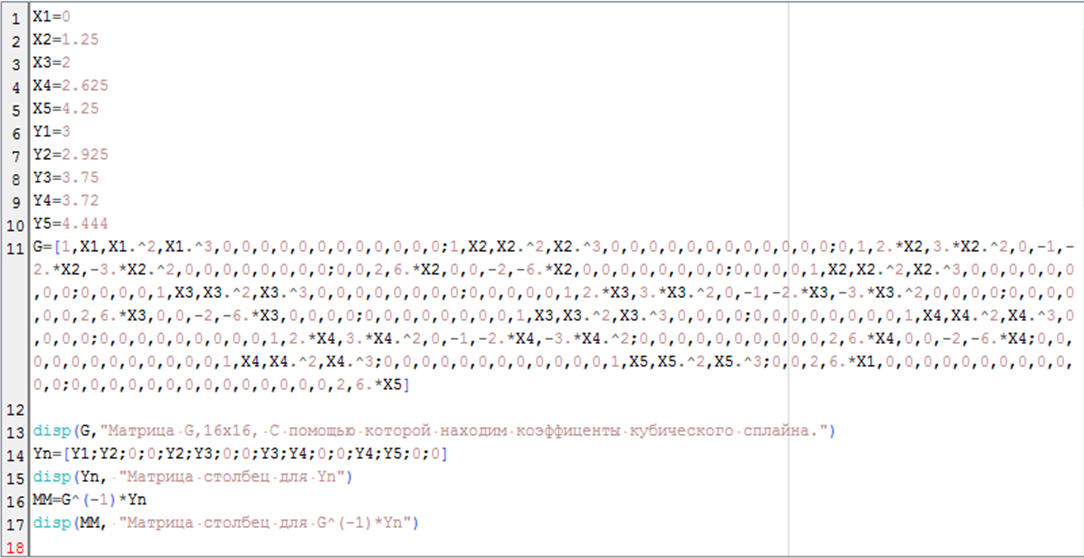
\includegraphics[width=0.9\linewidth]{123.PNG}} \\
\caption{1 часть скрипта для вычисления сплайна}
\end{figure}

\begin{figure}[H]
\center{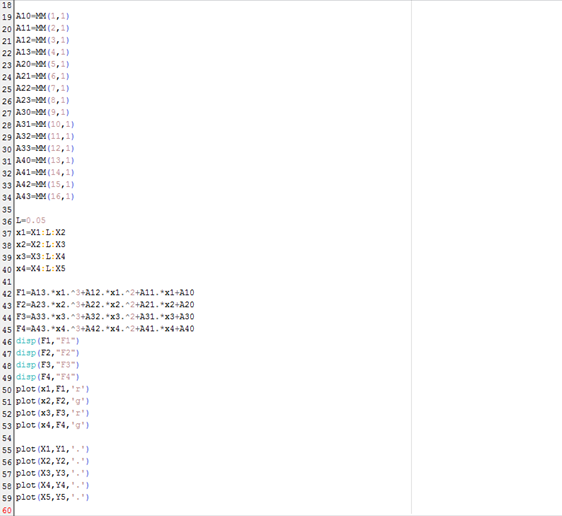
\includegraphics[width=0.9\linewidth]{2.PNG}} \\
\caption{2 часть скрипта для вычисления сплайна}
\end{figure}

\begin{figure}[H]
\center{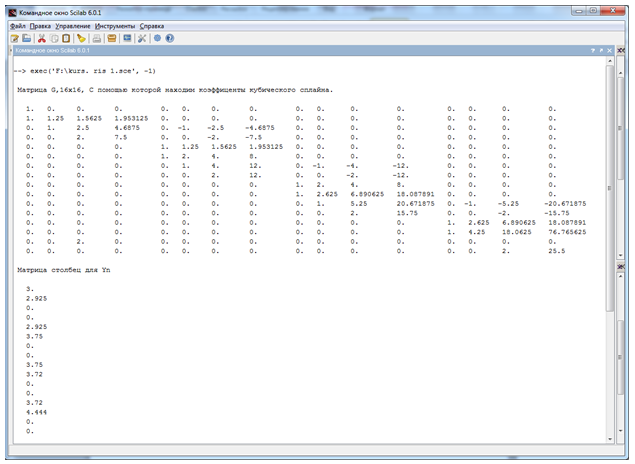
\includegraphics[width=0.9\linewidth]{3.PNG}} \\
\caption{Матрица }
\end{figure}

\begin{figure}[H]
\center{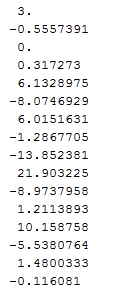
\includegraphics[width=0.3\linewidth]{4.PNG}} \\
\caption{Значения для коэффицентов $A_{ij}$}
\end{figure}

Окончательные уравнения сплайна
$$F_1=0,317x^3+0x^2-0,556x+3$$
$$F_2=-1,287x^3+6,015x^2-8,075x+6,133$$
$$F_3=1,211x^3-8,974x^2+21,903x-13,852$$
$$F_4=-0,116x^3+1,48x^2-5,538x+10,159$$

\begin{figure}[H]
\center{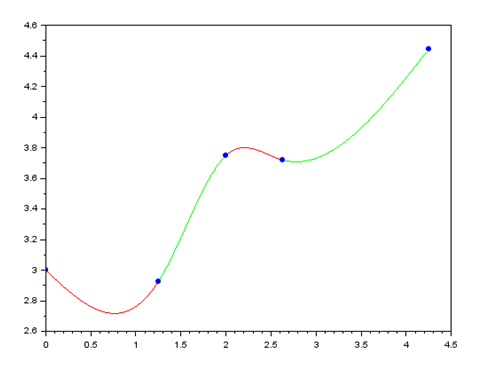
\includegraphics[width=0.9\linewidth]{5.PNG}} \\
\caption{Построение кубического сплайна}
\end{figure}

\subsection{Нахождение значения функции в тоxке Х=2,1}
Найдём значение функции в точке х=2,1
Подставим х=2,1 в полином данного промежумка 
$$F_3=1,211x^3-8,974x^2+21,903x-13,852$$
$$y_{(x=2,1)}=3,784$$

\newpage

\subsection{Оценка погрешности интерополяции в точке х=3.1}
{\bf Оценка погрешности интерполяции Эрмитовыми
кубическими сплайнами}
 Оценка погрешности интерполяции Эрмитовыми
кубическими сплайнами проводится после получения четвёртой производной функции. Далее вычисляем h -- из координаты х точки в которой вычисляется погрешность вычитаем координату ближайшей к ней точки $x_i$. После чего подставляем значения в формулу $P=\frac{1}{384}|f''''(x)|$



\end{document}














